%----------------------------------------------------------------------------------------
%	PACKAGES AND THEMES
%----------------------------------------------------------------------------------------

\documentclass[aspectratio=169]{beamer}
\mode<presentation> {
	
	\usetheme{Boadilla}
}
\definecolor{lmugreen}{RGB}{0, 136, 58}
\usecolortheme[named=lmugreen]{structure}
\usepackage{graphicx} % Allows including images
\usepackage{booktabs} % Allows the use of \toprule, \midrule and \bottomrule in tables
% \usepackage[english]{babel}
\usepackage[ngerman]{babel}  % Load German language support
\usepackage[utf8]{inputenc}
\usepackage{amsmath,amssymb} % math symbols
\usepackage{graphicx}
\usepackage{float}
\usepackage{tikz} % for DAGs
\usetikzlibrary{positioning, arrows, arrows.meta}
\usepackage[backend=biber,style=numeric]{biblatex}  % Numeric citations
\usepackage{hyperref} % for URLs
\newcommand{\gray}{\rowcolor[gray]{.90}}
\usepackage{verbatim}
\usepackage{textpos} % logo position
\usepackage[default]{sourcesanspro} % font type
\usepackage{cases} % math cases

\addbibresource{../literature.bib}  % Your exported .bib file

% Caption
\usepackage{caption}
\DeclareCaptionFont{tiny}{\tiny}
\captionsetup{font=scriptsize,labelfont=scriptsize,justification=centering}

% ToC
\AtBeginSection[]{
	\begin{frame}[noframenumbering, plain]
	\frametitle{Agenda}
	\setcounter{tocdepth}{1}
	\tableofcontents[currentsection]
\end{frame}
}
\newcommand{\FirstAgendaSlide}{
  \begin{frame}[plain]
    \frametitle{Agenda}
    \setcounter{tocdepth}{1}
    \tableofcontents[sectionstyle=show/show, pausesubsections=false]
  \end{frame}
}


% Remove navigation 
\beamertemplatenavigationsymbolsempty

% R 
\usepackage{listings}
\lstset{
language=R,
basicstyle=\scriptsize\ttfamily,
commentstyle=\ttfamily\color{gray},
backgroundcolor=\color{white},
showspaces=false,
showstringspaces=false,
showtabs=false,
tabsize=2,
captionpos=b,
breaklines=false,
breakatwhitespace=false,
title=\lstname,
escapeinside={},
keywordstyle={},
morekeywords={}, 
belowskip = -1.2 \baselineskip,
}

%----------------------------------------------------------------------------------------
%	TITLE PAGE
%----------------------------------------------------------------------------------------

\addtobeamertemplate{frametitle}{}{%
	\begin{textblock*}{100mm}(0.88\textwidth,-0.5cm)
		\includegraphics[height=1cm,width=2cm]{../figures/lmu_logo}
\end{textblock*}}

%\includegraphics[width=0.3\textwidth]{lmu_logo}
\vspace*{-1cm}

\title{Fair Machine Learning} 

\author{Juliet Fleischer} % Your name
\institute[LMU]{LMU} % Your institution as it will appear on the bottom of every slide, may be shorthand to save space
{

}
\begin{document}

{
\usebackgroundtemplate{\includegraphics[width=\paperwidth]{../figures/lmu-background.pdf}}
\begin{frame}
\begin{columns}
	\begin{column}{0.4\textwidth}
		\vspace{2.5cm}
		
		\textbf{\textcolor{white}{\Large Fair Machine Learning}}
		\vspace{1cm}
		
		\textcolor{white}{\footnotesize Juliet Fleischer \\
			\today}
	\end{column}
	\begin{column}{0.49\textwidth}
		\vspace{3cm}
		\begin{center}
			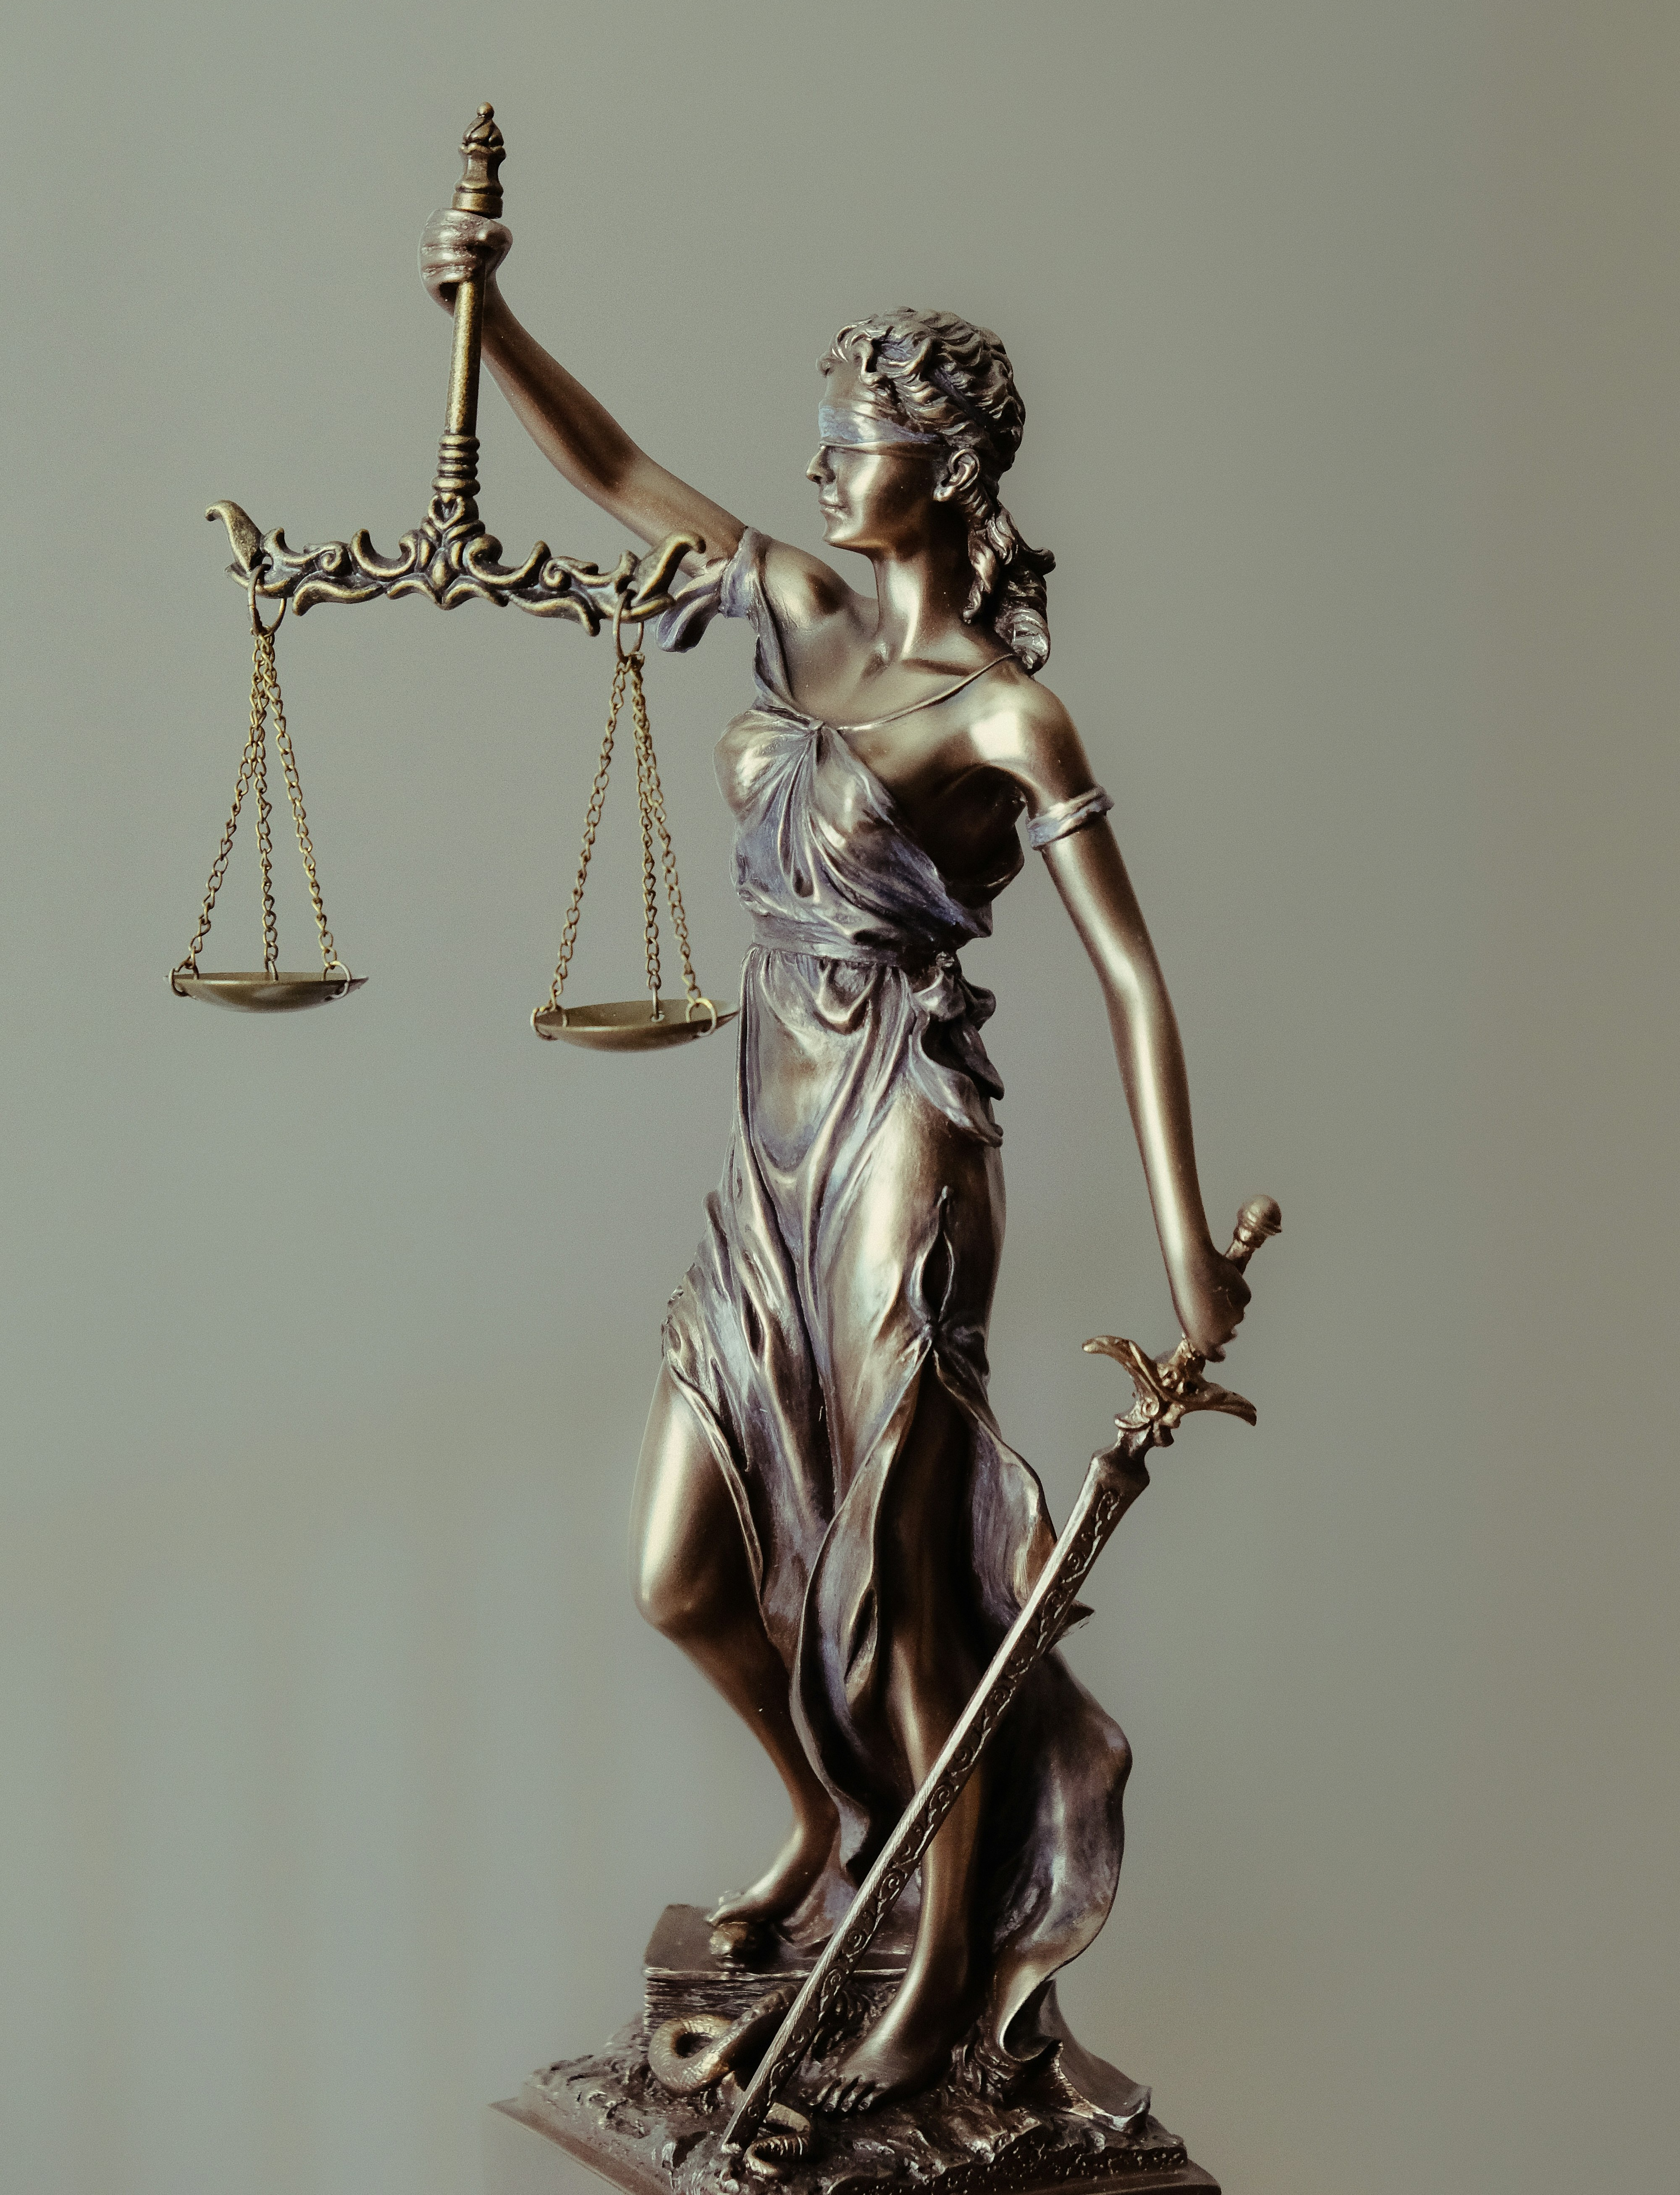
\includegraphics[width=0.55\textwidth]{../figures/fairness_title.jpg}
		\end{center}
	\end{column}
\end{columns}
\end{frame}
}
%----------------------------------------------------------------------------------------
%	PRESENTATION SLIDES
%----------------------------------------------------------------------------------------





\begin{frame}{Ist die Vorhersage fair?}
    % Full-width text
    \begin{itemize}
		\item<1-> Ziel: Kriminalitätsrate in NYC reduzieren
		\item<2-> Zielvariable: Straftat begangen  (0 = Nein, 1 = Ja)
        \item<3-> Trainingsdaten: vergangene Polizeistops
        \item<4-> Problem: Daten könnten vergangene Diskriminierung widerspiegeln (racial profiling,...) \\
		\onslide<5->$\Rightarrow$ Wie können wir sicherstellen, dass der Algorithmus gerecht entscheidet?
    \end{itemize}
\end{frame}

\FirstAgendaSlide

\section{Gruppen Fairness}
% Gruppen Fairness - Independence
\begin{frame}[t]{Gleiche Vorhersageraten zwischen Gruppen sind fair} % [t] aligns content at the top
	\begin{table}
        \begin{tabular}{lll}
            \toprule
            \color{orange}{Independence} & Separation & Sufficiency \\
            \midrule
            \color{orange}{$\hat{Y} \perp A$} & $\hat{Y} \perp A | Y$ & $Y \perp A | \hat{Y}$\\
            \bottomrule
        \end{tabular}
    \end{table}
	\begin{itemize}
		\item<2-> Verständnis von Fairness: Personen erfahren aufgrund ihrer Gruppenzugehörigkeit Diskriminierung
		\item<3-> Gruppenzugehörigkeit über \textbf{Protected Attribute (PA)} definiert
		\item<4-> Vorhersageraten zwischen Gruppen sollen gleich sein
		\item<6-> z.B. Statistical Parity \cite{verma2018} 	$$P(\hat{Y} = 1 | A = a) = P(\hat{Y} = 1 | A = b)$$ % 
	\end{itemize}
	\vspace*{-6cm}
	% include graphic only in frame 5
	\onslide<5>{
		\begin{center}
			\includegraphics[width=0.6\textwidth]{../figures/independence_02.png}
		\end{center}
	}
\end{frame}

% Gruppen Fairness - Separation
\begin{frame}[t]{Fairness anhand der Fehlermatrix konstruieren}
	\begin{table}
        \begin{tabular}{lll}
            \toprule
            Independence & \color{blue}{Separation} & \color{red}{Sufficiency} \\
            \midrule
            $\hat{Y} \perp A$ & \color{blue}{$\hat{Y} \perp A | Y$} & \color{red}{$Y \perp A | \hat{Y}$}\\
            \bottomrule
        \end{tabular}
    \end{table}
	\begin{columns}
		\column{0.5\textwidth}
		\raggedright  % Left-aligns text
		\begin{itemize}
			\item<2-> \textbf{Separation:} Fokus auf gleichen Fehlerraten zwischen Gruppen
			\item<5-> z.B. Predictive Equality \cite{verma2018} $$P(\hat{Y} = 1 | A = a, Y = 0) = P(\hat{Y} = 1 | A = b, Y = 0)$$
			\item<6-> \textbf{Sufficiency:} Zuverlässigkeit der Vorhersage soll gleich sein
			\item<7-> z.B. Predictive Parity \cite{verma2018} $$P(Y = 1 | A = a, \hat{Y} = 1) = P(Y = 1 | A = b, \hat{Y} = 1)$$
		\end{itemize}
		\column{0.5\textwidth}
		\onslide<4->{
			\begin{center}
				\renewcommand{\arraystretch}{1.5}  % Increase row height for a more square-like appearance
				\begin{tabular}{c|c|c|}
					& \color{blue}\(Y = 0\) & \color{blue}\(Y = 1\) \\
					\hline
					\color{red}\(\hat{Y} = 0\) & TN & FN \\
					\hline
					\color{red}\(\hat{Y} = 1\) & FP & TP \\
					\hline
				\end{tabular}
			\end{center}
		}
	\end{columns}
	\vspace*{-9cm}
	% include graphic only in frame 3
		\onslide<3>{
			\begin{center}
				\includegraphics[width=0.6\textwidth]{../figures/separation_01.png}
			\end{center}
		}
\end{frame}



% %Gruppen Fairness - Sufficiency
% \begin{frame}[t]{Zahlreiche Variationen von Gruppen-Metriken}
% 	\begin{table}
% 		\begin{tabular}{lll}
% 			\toprule
% 			Independence & Separation & {Sufficiency} \\
% 			\midrule
% 			$\hat{Y} \perp A$ & $\hat{Y} \perp A | Y$ & {$Y \perp A | \hat{Y}$}\\
% 			\bottomrule
% 		\end{tabular}
% 	\end{table}
% 	\begin{itemize}
% 		\item<2-> Sowohl Separation als auch Sufficiency können statt mit $\hat{Y}$ auch mit S definiert werden, z.B. Calibration 	$$P(Y = 1 | A = a, S = s) = P(Y = 1 | A = b, S = s)$$
% 		\item<3-> oder Well-calibration $$P(Y = 1 | A = a, S = s) = P(Y = 1 | A = b, S = s) = s$$
% 	\end{itemize}

% \end{frame}

\begin{frame}{Gruppenmetriken im Überblick}
	\begin{table}
		\begin{tabular}{lll}
			\toprule
			Independence & Separation & {Sufficiency} \\
			\midrule
			$\hat{Y} \perp A$ & $\hat{Y} \perp A | Y$ & {$Y \perp A | \hat{Y}$}\\
			\bottomrule
		\end{tabular}
	\end{table}
	\begin{itemize}
		\item<2-> Zahlreiche Variationen von Gruppen-Metriken \\ z.B. Calibration $P(Y = 1 | A = a, S = s) = P(Y = 1 | A = b, S = s)$
		\item<3-> Sufficiency nimmt Perspektive des Entscheidenden an \cite{castelnovo2022}
		\item<4-> Separation gut, wenn Y durch einen objektiv wahren Prozess entstanden ist \cite{castelnovo2022}
		\item<5-> Independence gut, wenn Form der Gleicheit erzwungen werden soll \cite{castelnovo2022}
	\end{itemize}
	\vspace*{0.5cm}
	\onslide<5->{
		\centering
		$\Rightarrow$ normalerweise nicht miteinander vereinbar
	}
\end{frame}


\section{Individuelle Fairness}
% Individuelle Fairness
\begin{frame}
    \frametitle{Gleicheit innerhalb der Gruppe vor Gleicheit zwischen Gruppen}
	\begin{itemize}
		\item Verständnis von Fairness: Fairness bedeutet, dass gleiche Personen gleich behandelt werden
	\end{itemize}
    \begin{enumerate}
		\item<2-> Fairness through Awareness \cite{dwork2012} (FTA)
        \begin{itemize}
            \item<3-> Lipschitz-Kriterium \cite{castelnovo2022}:
            \[
            d_Y(\hat{y_i}, \hat{y_j}) \leq \lambda {\color{orange}{d_X}}(x_i, x_j)
            \] 
            \item<4-> Definition des {\color{orange}Distanzmaßes $d_X$} im Feature Space ist eine Herausforderung
        \end{itemize}
        \item<5-> Fairness through Unawareness (FTU) = Blinding
        \begin{itemize}
            \item<6-> Vorgehensvorschrift: PA soll nicht im Entscheidungsprozess verwendet werden
            \item<7-> Keine eindeutige mathematische Definition, sondern verschiedene Ansätze zum Testen von FTU
            \item<8-> Problem der \textbf{Proxies} (Variablen, die mit PA hoch korreliert sind)
        \end{itemize}
    \end{enumerate}
\end{frame}


\section{Fairness Methoden}
% Fairness Methoden
\begin{frame}
	\frametitle{Wie sorgen wir für algorithmische Fairness?}
	\begin{itemize}
		\item<1-> Preprocessing \cite{caton2024}: Daten vor dem Training bearbeiten \\ z.B. (Re-)Sampling
		\item<2-> Inprocessing \cite{caton2024}: Trainingsprozess anpassen, Optimierungsproblem modifizieren \\ z.B. Regularisierung
		\item<3-> Postprocessing \cite{caton2024}: Vorhersagen nach dem Training bearbeiten \\ z.B. Thresholding
		\item<4-> UQ und XAI Methoden können hier auch helfen!
	\end{itemize}
\end{frame}


\section{Bias und die Feedback Loop}
% Quellen von Bias
\begin{frame}{Woher kommt Bias?}
	% insert an image
	\begin{figure}
		\centering
		\includegraphics[width=0.7\textwidth]{../figures/bias_loop.png}
		\caption{Quellen von Bias in der Daten, Nutzer, Algorithmus Feedback Loop \cite{mehrabi2022}}
	\end{figure}
\end{frame}

% Fazit und Ausblick
\begin{frame}{Wie geht es weiter?}
	\begin{itemize}
		\item<1-> Binäre Klassifikation, ein PA ist simpelster Fall
		\item<2-> In Praxis eher mehrere PAs und vielfältige Aufgaben\\ $\rightarrow$ regression, unsupervised learning, ...
		\item<3-> Es gibt (noch) nicht, die \textbf{eine} Definition von Fairness
	\end{itemize}
\end{frame}

\begin{frame}[allowframebreaks]
	\frametitle{Referenzen}
	\printbibliography
\end{frame}

% Extra slides
\section{Extra Folien}

% Anmerkungen zu observational Fairness Metriken
\begin{frame}{Mögliche Diskussionspunkte}
	\begin{itemize}
		\item Sind Gruppen-Metriken zu simplistisch gedacht? spiegeln einfach Verteilung von Y, A, $\hat{Y}$, (X) in den Daten wider \cite{corbett-davies} $\rightarrow$ keine Kausalität oder externe Faktoren
		\item Folgen von Fairness Interventionen nicht sicher - profitiert die geschützte Gruppe wirklich?
		\item Welche Vor- und Nachteile haben gruppenbasierte gegenüber individuellen Fairnessmetriken? Sind die beiden miteinander vereinbar?
		\item Welche Möglichkeiten gibt es für UQ und XAI zu Fairness im machine learning beizutragen?
	\end{itemize}
\end{frame}

% Details: Individuelle Fainress
\begin{frame}{Weitere Möglichkeiten FTU zu messen}
	\begin{align*}
		\text{consistency} &= 1 - \frac{1}{n} \left( \sum_{i=1}^n \left| \hat{y}_i - \frac{1}{k} \sum_{x_j \in kNN(x_i)} \hat{y}_j \right| \right) \hfill (1) \\
	\end{align*}
		
	\begin{align*}
		\frac{1}{n_1 n_2} \sum_{a_i=1, a_j=0} e^{-\text{dist}(x_i, x_j)} \left| \hat{y}_i - \hat{y}_j \right| \hfill (2)
	\end{align*}		
\end{frame}

% Kausale Fairness
\begin{frame}{Ist die Gruppenzugehörigkeit der Grund für die Festnahme? \\ - kausale Definitionen}
    \begin{columns}
        \column{0.4\textwidth}
        \centering
		\begin{tikzpicture}[node distance=3cm, >=stealth', thick]
			% Nodes
			\node (Race) [circle, draw, fill=blue!20] {Race};
			\node (Precinct) [circle, draw, fill=yellow!20, right of=Race] {Precinct};
			\node (Arrest) [circle, draw, fill=red!20, below of=Precinct] {Arrest};
		
			% Arrows
			\draw[->] (Race) -- (Arrest);
			\draw[->] (Precinct) -- (Arrest);
		\end{tikzpicture}
		
        \column{0.4\textwidth}
		\begin{itemize}
			\item Gruppen Fairness: FACE, FACT (on average or on conditional average level) \cite{Zafar2017PPNFC}
			\item Individuelle Fairness: counterfactual fairness, path-based fairness \cite{kusner}
		\end{itemize}
    \end{columns}
\end{frame}

% Weitere Resourcen
\begin{frame}{Ressourcen für Fairness in Machine Learning}
    \begin{itemize}
        \item Interaktives Tool: \url{https://research.google.com/bigpicture/attacking-discrimination-in-ml/}
        \item Einführung in Fairness mit mlr3.fairness: \url{https://journal.r-project.org/articles/RJ-2023-034/}
        \item Fairness and Machine Learning Buch: \url{https://fairmlbook.org/}
    \end{itemize}
\end{frame}


% Weitere Infos zu den Daten
\begin{frame}{POC werden überproportional häufig gestoppt}
    \text{Verteilung der Ethnie in NYC (2023)} \\
    \url{https://www.census.gov/quickfacts/newyorkcitynewyork}

    \vspace{0.3cm}  % Add some space before the table
	% add a title above the table

    \begin{table}
        \centering  % Center the table
		\caption{Verteilung der Ethnie in SQF Daten}
        \begin{tabular}{ll}
            \toprule
            race & prop \\
            \midrule
            \color{orange}{BLACK} & 58.61\% \\
            \color{orange}{WHITE HISPANIC} & 20.32\% \\
            \color{orange}{BLACK HISPANIC} & 10.13\% \\
            WHITE & 5.48\% \\
            OTHER & 2.67\% \\
            NA & 2.79\% \\
            \bottomrule
        \end{tabular}
    \end{table}
\end{frame}




\end{document}


